\documentclass{article}
\usepackage[utf8]{inputenc}
\usepackage{graphicx}

\author{Bijan Varjavand}
\title{LabNotebook}
\date{April 11, 2017}

\begin{document}

\maketitle

\section{Objectives}

The objective for our group this day was to learn more about the thermoelectric effect.

\section{Setup}

This lab was not set up very well, as there was no push to get the students to start work. As a result, a few students were lost and weren't able to do the lab.

\subsection{Materials}

We used blocks of aluminum. This is because aluminum has very high thermal conductivity.

\subsection{Tools}

We used an electric system which was able to become a heat pump or a heat engine.

\section{Procedure}

First, we operated the apparatus in heat pump mode. The energy was pumped from one aluminum block to another. Once a temperature gradient was reached, the heat pump was switched to become a heat engine.

\section{Results}

We measured the input power from the power supply in heat pump mode. We also measured the power generated from the heat engine. A figure showing the relationship between the two is shown below.

\begin{figure}[h!]
\centering
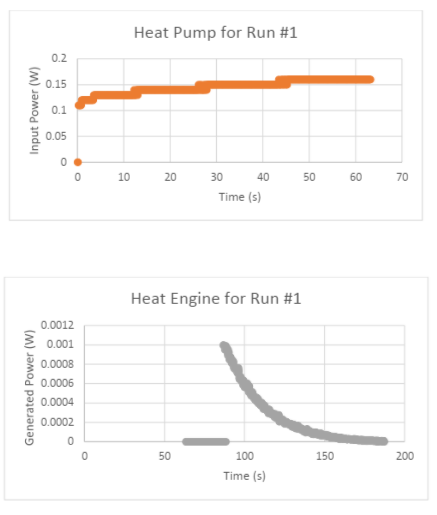
\includegraphics[scale=1.2]{thermo.png}
\end{figure}

\section{Observations}

Simply taking integrals of the two graphs gives us the energy from each process. Comparing a ration between these two energies gives us percent useful work which was about 2.7\%. This is very bad, since aluminum gives off heat too easily.

\end{document}